%% no need for  \DeclareGraphicsExtensions{.pdf,.eps}

\documentclass[12pt,letterpaper,english]{article}
\usepackage{times}
\usepackage[T1]{fontenc}
\IfFileExists{url.sty}{\usepackage{url}}
                      {\newcommand{\url}{\texttt}}

\usepackage{babel}
%\usepackage{noweb}
\usepackage{Rd}

\usepackage{Sweave}

%\VignetteIndexEntry{Performance Attribution from Bacon}
%\VignetteDepends{PerformanceAnalytics}
%\VignetteKeywords{returns, performance, risk, benchmark, portfolio}
%\VignettePackage{PerformanceAnalytics}

%\documentclass[a4paper]{article}
%\usepackage[noae]{Sweave}
%\usepackage{ucs}
%\usepackage[utf8x]{inputenc}
%\usepackage{amsmath, amsthm, latexsym}
%\usepackage[top=3cm, bottom=3cm, left=2.5cm]{geometry}
%\usepackage{graphicx}
%\usepackage{graphicx, verbatim}
%\usepackage{ucs}
%\usepackage[utf8x]{inputenc}
%\usepackage{amsmath, amsthm, latexsym}
%\usepackage{graphicx}

\title{Maximum Loss and Maximum Drawdown in Financial Markets}
\author{R Project for Statistical Computing}

\begin{document}
\Sconcordance{concordance:ShaneAcarMaxLoss.tex:ShaneAcarMaxLoss.Rnw:%
1 47 1 1 5 1 4 21 1 1 2 1 0 2 1 4 0 1 2 3 1}


\maketitle


\begin{abstract}
The main concern of this paper is the study of alternative risk measures: namely maximum loss and 
maximum drawdown. Both statistics have received little attention from academics despite their  extensive use by proprietary traders and derivative fund managers. 
Firstly, this paper recalls from previously published research the expected maximum loss under the  normal random walk with drift assumption. In that case, we see that exact analytical formulae can be established. The expected maximum loss can be derived as a function of the mean and standard deviation of the asset. For the maximum drawdown, exact formulae seems more difficult to establish. 
Therefore Monte-Carlo simulations have to be used. 
\end{abstract}



\section{Background}

The model is focused on concept of drawdown measure which is in possession of all properties of a deviation measure,generalization of deviation measures to a dynamic case.Concept of risk profiling - Mixed Conditional Drawdown (generalization of CDD).Optimization techniques for CDD computation - reduction to linear programming (LP) problem. Portfolio optimization with constraint on Mixed CDD
The model develops concept of drawdown measure by generalizing the notion
of the CDD to the case of several sample paths for portfolio uncompounded rate
of return.


\section{Maximum Drawdown}
Unfortunately, there is no analytical formulae to establish the maximum drawdown properties under the random walk assumption. We should note first that due to its definition, the maximum drawdown divided by volatility is an only function of the ratio mean divided by volatility. 
\begin{equation}
MD / \sigma =  Min \frac{ \sum_{j=1}^{t} X_{j}}{\sigma} = F(\frac{\mu}{\sigma}) \\
\end{equation}

Such a ratio is useful in that this is a complementary statistic to the return divided by volatility ratio. To get some insight on the relationships between maximum drawdown per unit of volatility and mean  return divided by volatility, we have proceeded to Monte-Carlo simulations. We have simulated cash flows over a period of 36 monthly returns and measured maximum drawdown for varied levels of  annualised return divided by volatility varying from minus two to two by step of 0.1. The process has  been repeated six thousand times.

\section{Usage}
Figure below illustrates the average maximum drawdown as well as the quantiles 85\%, 90\%, 95\%, 99\%.For instance, an investment exhibiting an annualised return/volatility equal to -2 should experience on average a maximum drawdown equal to six times the annualised volatility.

Other observations are that:maximum drawdown is a positive function of the return /volatility ratio ,confidence interval widens as the return/volatility ratio decreases.This means that as the return/volatility increases not only the magnitude of drawdown decreases but the confidence interval as well. In others words losses are both smaller and more predictable.

\begin{Schunk}
\begin{Sinput}
> library(PerformanceAnalytics)
> data(edhec)
> chart.AcarSim(edhec)
\end{Sinput}
\end{Schunk}
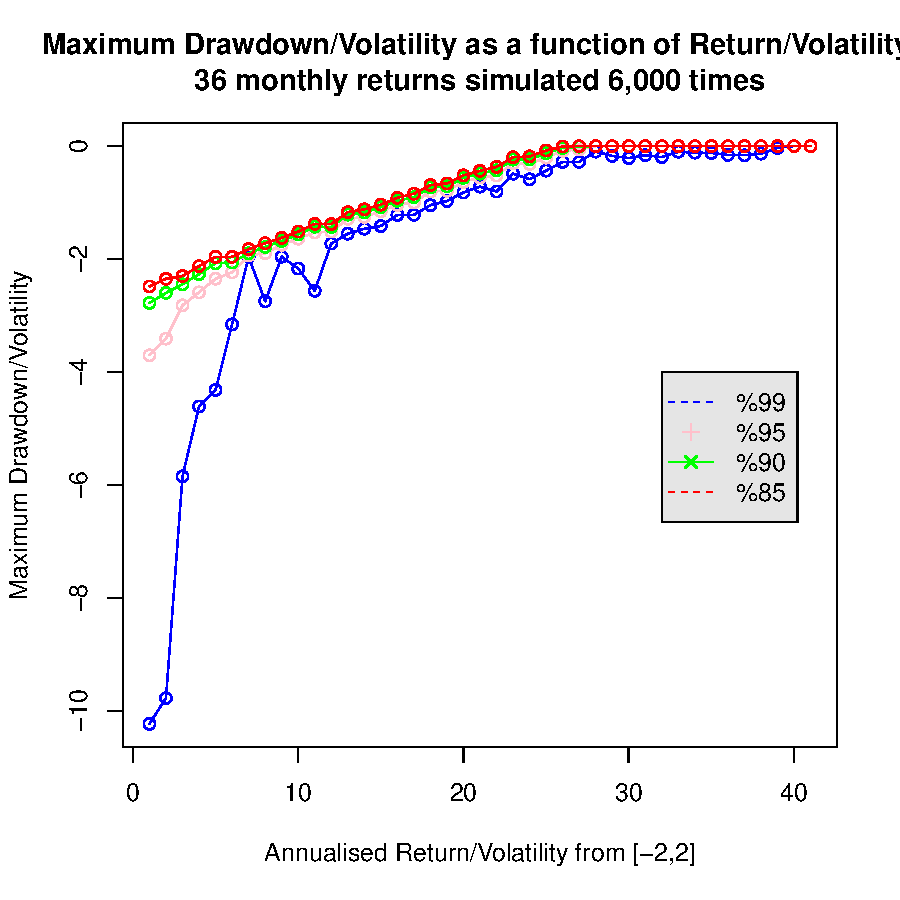
\includegraphics{ShaneAcarMaxLoss-003}



\end{document}
